\section{El LSD sobre el cerebro.}

La introducción de entidades exógenas como el LSD u otras sustancias al organismo produce un desequilibrio con toda clase de consecuencias.

\subsection{¿Qué es una droga?}

Los organismos consumen diversas sustancias del entorno. Algunas son asimiladas inmediatamente y convertidas en materia y energía o producen excrementos. Llamamos a estas alimentos. Otras no lo son tan fácilmente: por condiciones genéticas, el cobre puede acumularse en el hígado con consecuencias graves (enfermedad de Wilson). Pero otras sustancias, en lugar de acumularse, desencadenan reacciones inmensas sobre el organismo. Estas son de especial importancia en medicina, pues al ser similares en estructura y/o función a sustancias endógenas al organismo, pueden ser utilizadas para regularlo directa o indirectamente.

Muchas sustancias pueden servir entonces como tratamiento para distintas enfermedades (como ocurre con la insulina para la diabetes). Pero por su misma naturaleza, su presencia en niveles altos en el cuerpo puede también resultar tóxica: la aspirina por ejemplo es letal en cantidades de unos 250 miligramos por kg de peso corporal (mg / kg). Por supuesto lo letal no es la aspirina en sí, sino la dosis respecto de la medida del peso corporal. Es esta doble acción de remedio y veneno la que describe la palabra griega \textit{phármakon} ($\phi\acute{\alpha}\rho\mu\alpha\kappa o\nu$). Era un hecho incluso entonces que la distinción entre remedio y veneno no depende de la sustancia, sino de la dosis.

Entre los no-alimentos encontramos sustancias que no solo actúan de manera somática (como el cianuro de potasio o el acetaminofén), sino que también inciden sobre el sistema nervioso, afectando a la percepción y la emoción (entendida como las reacciones psicofisiológicas internas del individuo ante estímulos importantes). A estas sustancias las llamamos \textit{drogas}.

Es importante notar que el término \enquote{droga} es polisémico, y a veces se usa para denominar exclusivamente a sustancias con efecto sobre el SN, mientras que otras se emplea para referirse a cualquier cuerpo químico utilizado en medicina (la palabra \enquote{\textit{drug}} recibe este uso particularmente en la lengua inglesa).

Por último es importante reconocer que muchas drogas son ilegales y, como tal, el término guarda otro significado en el ámbito del derecho. Históricamente la relación de la humanidad con las drogas ha sido asunto de controversia (véase el ejemplo del vino en la Antigua Roma), y de manera cultural o sistemática se ha perseguido el uso de unas u otras. En torno al último tercio del siglo XX se establece una normativa más estricta en países como Estados Unidos con el Controlled Substances Act y \enquote{droga} pasa a designar a cualquier sustancia así designada por este estatuto.

Para evitar ambigüedades, en este documento emplearemos las siguientes definiciones:

\begin{itemize}
	\item Fármaco: cualquier sustancia utilizada como tratamiento para una enfermedad.
	\item Droga: cualquier sustancia que interactúa con el sistema nervioso produciendo cambios en la percepción y la emoción.
\end{itemize}

\subsection{Terminología}

Existe un conjunto de términos asociados tanto a drogas como a fármacos que definimos cuantitativa y cualitativamente. En primer lugar tenemos aquéllos referentes a la dosis. Distintos organismos difieren en sus características particulares y no reaccionarán de la misma manera a dosis iguales, es así que nuestras afirmaciones serán estadísticas y no concretas.

Es común administrar una dosis determinada a una población y observar sus efectos. La \textit{dosis efectiva media} (ED50) es aquélla que produce los efectos deseados sobre el 50\% de los individuos a los que se da (puede haber distintas dosis efectivas dependiendo de los efectos que se desee producir). La \textit{dosis letal media} (LD50) es aquélla suficiente para acabar con la vida del mismo porcentaje de población. De estas dos se extrae el margen de seguridad, que es la proporción entre dósis activa media y dósis letal media.

Tanto fármacos como drogas pierden parcial o totalmente su efecto con el uso continuado, este fenómeno es conocido como \textit{tolerancia}. Repetidas dosis diarias de aspirina generan una tolerancia que la hace mucho menos efectiva. Esta capacidad de adaptación del cuerpo no es igual para todas las sustancias, por lo que la tolerancia que induce cada una ha de ser estudiada individualmente.

En la literatura relacionada a las drogas se suele usar a la tolerancia como medida sinónima de propensión al abuso. Si bien razonable, se puede matizar. Ciertamente una droga como la heroína generará una rápida adaptación, por lo que el usuario, para sentir los mismos efectos, habrá de dejar un margen entre uso y uso o, como es común, aumentar la dosis. La adaptación del organismo al fármaco sin embargo no es pareja, y un individuo puede dejar de percibir los efectos relajantes de un opioide pero seguir sufriendo la misma depresión respiratoria. Un aumento de la dosis en este caso plantea el riesgo de intoxicación aguda. Incluso si se consigue una adaptación pareja, el uso continuado de la droga termina generando una intoxicación crónica, como es habitual en casos de alcoholismo. Un menor grado de adaptación implica límites de toxicidad más rígidos, reduciendo el riesgo de intoxicación crónica pero haciendo más fácil alcanzar dosis perjudiciales o letales.

Que el cuerpo se adapte a fármacos supone cambios metabólicos internos que hacen que el organismo necesite la presencia de la sustancia para mantener su equilibrio. Se dice entonces que el cuerpo ha generado \textit{dependencia} a la sustancia. Cuando la sustancia es eliminada --- por ejemplo por interrumpirse su uso continuado --- se produce un fenómeno de desestabilización que se manifiesta en reacciones mensurables conocido como \textit{síndrome de abstinencia}. Uno empieza a vislumbrar aquí los mecanismos biológicos que conducen a la adicción, esto es, la búsqueda compulsiva de nuevas dosis, sin embargo hemos de hacer un comentario adicional al respecto.

\newpage

\subsection{Adicción y dependencia.}

Mismos estímulos provocan distintas respuestas dependiendo de variables internas como el hambre o el estado anímico. Ante la presencia de agua y alimento, el depredador prioriza aquélla necesidad más urgente en ese momento. A ese conjunto de variables internas y su influencia sobre las externas lo llamamos \textit{motivación}. La mayoría de las motivaciones buscan saciar un desequilibrio interno a corto plazo como la sed, pero algunas expanden su vista a imperativos biológicos como la perpetuación de la especie.

Cuando un agente estimula los sistemas de recompensa del cerebro de manera artificial – llegando a predominar sobre recompensas naturales, incluso en detrimento físico o psicológico del individuo – se dice que existe una \textit{adicción}. La adicción se define como un síndrome crónico caracterizado por la búsqueda compulsiva de cierta droga, incluso ante consecuencias negativas físicas y personales.

Este fenómeno es estudiado principalmente en animales. Por ejemplo, cuando una rata es encerrada y provista de una palanca con la que estimular eléctricamente ciertas regiones de su cerebro, la rata tirará de la palanca incluso en condiciones de inanición, llegando a ignorar la comida que se le ofrezca. La persecución de una mete artificial en perjuicio de la necesidad biológica forma un paralelo interesantísimo con la adicción a drogas. Comprender las vicisitudes de la adicción implica entender los sistemas de recompensa del cerebro, algo que aún se está investigando.

Al analizar la actividad cerebral que suscitan distintos comportamientos hedónicos observamos que ciertas regiones muy concretas se activan de manera consistente. Una de estas regiones es el \textit{área tegmental ventral} (VTA por sus siglas en inglés), una región del cerebro con muchas proyecciones al \textit{núcleo accumbens} (NAc). La comunicación entre estas dos zonas se realiza por medio de un neurotransmisor llamado \textit{dopamina}, y las neuronas que la utilizan son \textit{dopaminérgicas} (Figura \ref{ratbrain}).

Algunas drogas como la cocaína o las anfetaminas son capaces de fortalecer la transmisión dopaminérgica, incrementando la actividad de los sistemas de recompensa como el de la VTA. Estas drogas no solo producen adicción física por su síndrome de abstinencia, sino que, debido a esta perturbación neuronal, causan también adicción psicológica.

\begin{figure}[H]
	\centering
	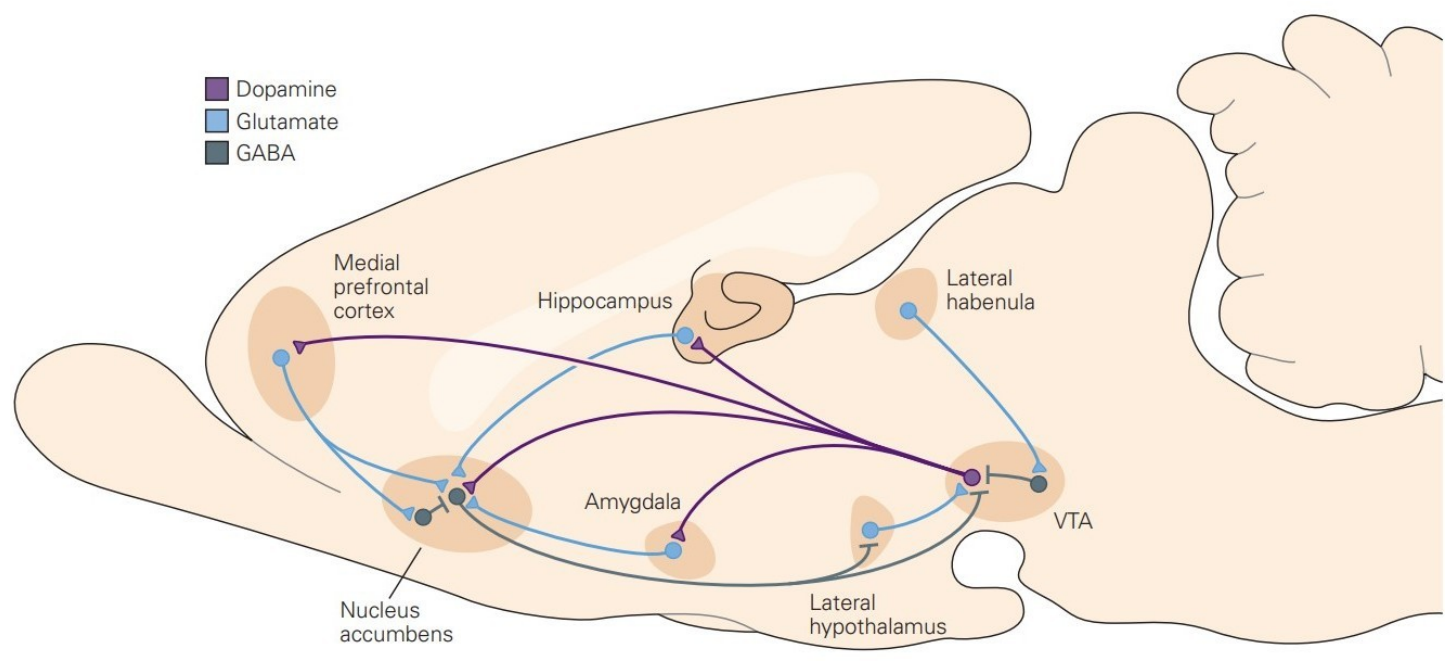
\includegraphics[width=\linewidth]{media/8-ratbrain.png}
	\caption{Esquema de proyecciones de la VTA en el cerebro de un ratón. Al activarse la VTA, neuronas dopaminérgicas (en morado) forman proyecciones excitatorias hacia distintas partes del cerebro (hipocampo, amígdala, NAc...) produciendo la emoción de recompensa.}
	\label{ratbrain}
\end{figure}

Esta explicación de la adicción sin embargo sigue sin ser completamente sólida. Identificar la dopamina con un \enquote{neurotransmisor del placer} es incorrecto. En ocasiones la dopamina señaliza respuestas negativas, y estudios más recientes asocian su liberación a un \enquote{error en la predicción}.

Además, la activación de neuronas dopaminérgicas es solo uno de los componentes de todos los procesos neuronales que ocurren durante la emoción de recompensa. Ratas carentes de dopamina aún exhiben comportamientos hedónicos ante el azúcar y la cocaína, lo que indica que este neurotransmisor no es el único factor relevante.

Peor aún, el patrón de comportamiento de realizar algo repetidamente incluso en detrimento propio puede aplicarse a conductas como el juego, la comida o el sexo, áreas complicadísimas de estudiar, pues es imposible construir un modelo humano a partir de una rata con adicción a ir de compras. Hasta en roedores es difícil hallar patrones deterministas: grupos de ratones no desarrollan adicción a la cocaína en las mismas proporciones estando totalmente aislados que dentro de \enquote{ambientes enriquecidos} dotados de compañeros, tubos de polietileno y pelotas.

¿Qué paralelismos se pueden trazar entre el comportamiento de una rata y el de un humano? ¿Cómo se manifiesta la adicción a escala neuronal y cómo se relaciona realmente a las drogas? Nos topamos con el mantra repetido durante toda investigación neurocientifica: no lo sabemos. Desprovistos de afirmaciones universales, nos vemos obligados a analizar los efectos concretos del LSD.

\newpage

\subsection{Farmacología del LSD.}

La dietilamida del ácido lisérgico es una droga semisintética derivada del ácido lisérgico extraído del ergot. Posee cuatro estereoisómeros, es decir, cuatro sustancias hermanas estructuralmente: l- y d- LSD y l- y d- iso-LSD. Solo el d-LSD es psicoactivo, y es al que nos referimos al decir \enquote{LSD}. Es hidrosoluble y se derrite a 83°C, y debido a su fragilidad ante la luz, la temperatura y la humedad suele ser conservado en su forma de sal de tartrato. Debido a su alta biodisponibilidad, la vía de administración más común es la oral. Originalmente se realizaba a través de ampollas, pero se popularizó el consumo a través de papeles secantes o terrones de azucar bañados y colocados sobre la lengua. Distintas dosis de LSD configuran distintos efectos.

En un individuo de entre 50 y 70 kg de peso, la mínima dosis reconocible es de 25 $\mu$g y produce algunas alteraciones cognitivas. La dosis estándar está entre 70 y 100 $\mu$g, y produce una acción de 6 a 10 horas, ya con efectos visionarios. A partir de 300 $\mu$g comienzan las dosis altas, con efectos intensos durante más de 10 horas.

La dosis letal media en distintos animales está entre 0.3 y 16.5 mg / kg, siendo 1 mg / kg en monos. No se ha encontrado la dosis letal en humanos, pues no se conocen casos de muertes por LSD. En una ocasión ocho individuos confundieron LSD con cocaina y consumieron una dosis altísima, hallando 1-7 mg de la sustancia por cada 100 mL de su sangre. Sufrieron de estados comatosos, hipertermia, vómitos, sangrados gástricos y problemas respiratorios, pero con tratamiento hospitalario, todos sobrevivieron sin secuelas. Es preciso afirmar entonces que el margen de seguridad del LSD es extraordinariamente alto.

El LSD presenta una tolerancia elevadísima. Después de dosis de entre 5 y 100 microgramos administradas durante 3 a 6 días, los voluntarios desarrollan una fuerte tolerancia. Esta desaparece en torno a los 4 días sin uso. Más allá de la tolerancia, existe un consenso general en que el LSD no es adictivo, es decir, no produce los comportamientos de búsqueda compulsiva de más dosis.

Se observa que esta sustancia tiene unas propiedades excepcionales, sin embargo que sea farmacológicamente segura no implica que su uso en general sea seguro. Existen casos documentados de autolesión y suicidio bajo los efectos de esta droga, si bien el número es reducido. Más detalles al respecto se dan en el capítulo sobre su historia contemporánea.

\newpage

\subsection{Efectos del LSD.}

Una dosis estándar de LSD altera de manera significativa el estado de consciencia, con una tendencia a la euforia, es decir, un intenso estado de felicidad y bienestar; un impulso en la capacidad de introspección y la estimulación de procesos Freudianos primarios, es decir, los deseos instintivos se desatan, inhibiendo la influencia del ego y la sociedad sobre el individuo. El efecto más característico son las alteraciones en la percepción como ilusiones, visiones, pseudoalucinaciones, sinestesias --- la capacidad de cruzar sentidos --- y alteraciones en el pensamiento y la percepción temporal. Mención especial merecen los cambios que provoca sobre la percepción de uno mismo y la función del ego. El LSD (especialmente en dosis altas) debilita la frontera que separa al \textit{yo} del resto del mundo, un fenómeno conocido como \enquote{disolución} o \enquote{muerte del ego}.

La potencia inigualada del LSD es un arma de doble filo, pues al igual que es capaz de proporcionar una buena experiencia y efectos psicológicos positivos a largo plazo, también puede provocar experiencias traumáticas (llamadas coloquialmente \enquote{malos viajes}) con efectos negativos como cambios de humor y, a veces, escenas retrospectivas que pueden resultar nocivas. Es difícil estudiar los efectos del LSD en el pensamiento, pues no podemos introducirnos en la mente de nadie y la dosis estándar ya es suficiente para dificultar la comunicación durante los experimentos. Se puede decir que el efecto del LSD reduce la destreza en pruebas de atención y concentración, habilidades psicomotoras y aritméricas, memoria visual y noción temporal – se tiende a sobreestimar los intervalos temporales. Los procesos de aprendizaje no se ven afectados. Ciertas interpretaciones argumentan que las funciones intelectuales sufren un regreso a un estado más temprano de desarrollo. No se conoce ninguna facultad perjudicada de manera crónica por el uso de LSD. En muchas personas produce mareos y agitación interna.

\subsection{Mecanismo de acción: el sistema serotoninérgico.}

La serotonina (también denominada 5-hidroxitriptamina o 5-HT) es un neurotransmisor que se produce a partir del triptófano en pocas neuronas (contadas en millares). Estas neuronas se ubican principalmente en los \textit{núcleos del rafe} del mesencéfalo, y proyectan sus conexiones a regiones como el hipocampo, la corteza cerebral, el NAc y núcleos dopaminérgicos como la VTA, entre otras (Figura \ref{pathways}). Es particularmente importante la conexión de los núcleos del rafe con el \textit{locus coeruleus} (LC), pues esta región se encarga de la liberación de noradrenalina y tiene conexiones con el cerebelo, el tálamo, el hipotálamo, la corteza y el hipocampo.

Es evidente que, a pesar de ser reducidas en número, las abundantes conexiones salientes de las neuronas serotoninérgicas (hasta 500.000 por neurona) hacen de la 5-HT un neurotransmisor crucial en procesos tan diferentes como la regulación del ánimo, la temperatura corporal y hasta el tracto gastrointestinal. La deficiencia en niveles de serotonina se asocia a trastornos depresivos, que son tratados con varias formas de psicoterapia y fármacos antidepresivos (normalmente inhibidores selectivos de recaptación de serotonina o SSRIs, como la fluoxetina y la sertralina).

El sistema serotoninérgico está también relacionado con el filtro de información en el cerebro. No todos los estímulos del medio son igual de importantes, y algunos --- como el sonido del oleaje --- son continuos y repetitivos, por lo que no merecen atención constante. El cerebro tiene una capacidad de procesamiento limitada, por lo que automáticamente descarta esta información para dejar espacio a otra más valiosa, evitando además una sobrecarga sensorial. Una alteración en este sistema de cribado podría explicar los efectos estimulantes y alucinógenos del LSD.

La estructura molecular del LSD es similar a la de la serotonina, lo que le permite unirse a algunos de sus receptores, aunque con menos fuerza que la propia serotonina (se dice que es un \textit{agonista parcial}). Esta interacción altera el comportamiento del sistema serotoninérgico, aunque no se conoce plenamente cómo. Las neuronas del sistema serotoninérgico cuentan con 14 receptores de serotonina distintos (y se teoriza un 15$^\circ$), siendo algunos inhibitorios y otros excitatorios, y la gran mayoría metabotrópicos (es decir, que no controlan directamente la apertura de un canal, sino que modulan la actividad de la neurona por medio de segundos mensajeros). Estos receptores se nombran como \enquote{5-HT$_{\textrm{XY}}$} (receptor de serotonina Y de la clase X).

Concretamente actúa como agonista parcial en los receptoers 5-HT$_{\textrm{1A}}$, 5-HT$_{\textrm{2A}}$ y 5-HT$_{\textrm{2C}}$, pero también sobre receptores de otros neurotransmisores como el dopaminérgico D$_2$ y el adrenérgico $\alpha_2$. Un efecto secundario de estimular los receptores 5-HT$_{\textrm{2A}}$ es la activación de transmisión glutamatérgica en la corteza frontal. Este es un patrón clave compartido por el LSD y otros alucinógenos serotoninérgicos, y se cree que esta activación podría causar una perturbación en los sistemas de filtro de procesos sensoriales y cognitivos. La tolerancia podría ocurrir debido a una reducción en la densidad de receptores 5-HT$_{\textrm{2A}}$.

\begin{figure}[H]
	\centering
	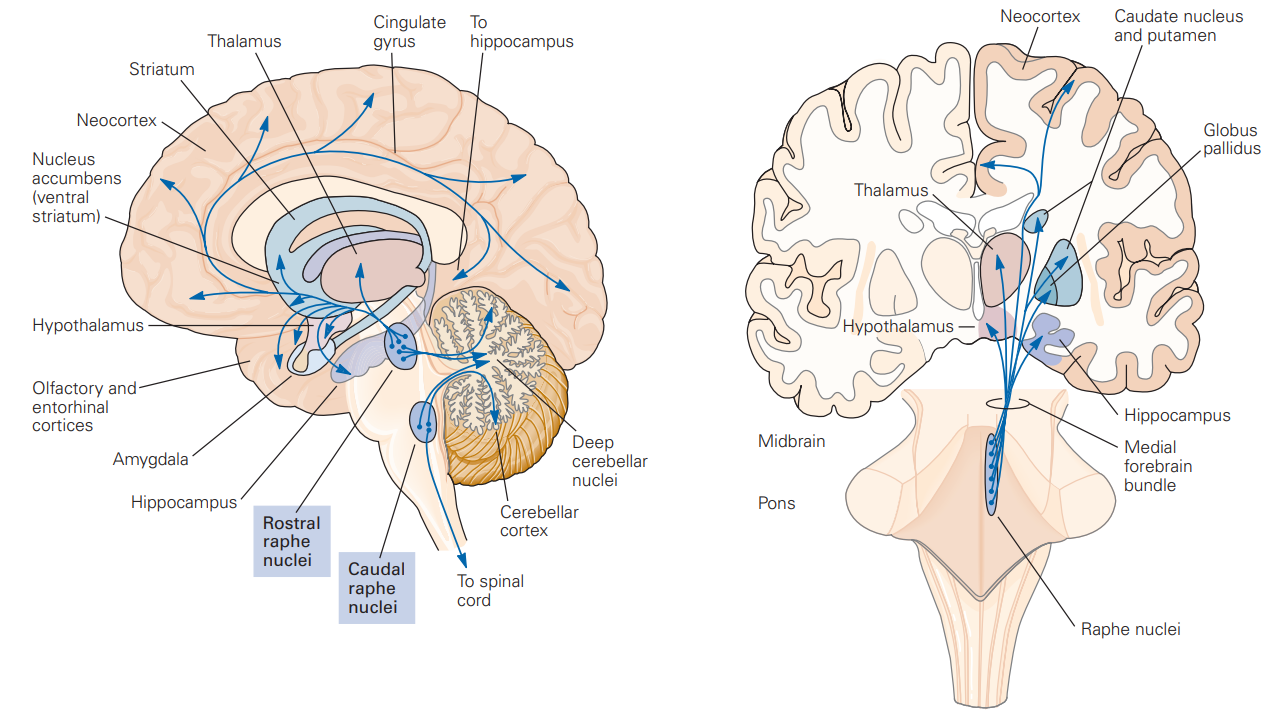
\includegraphics[width=\linewidth]{media/9-pathways.png}
	\caption{Rutas serotoninérgicas encefálicas. Las neuronas serotoninérgicas nacientes de los núcleos del rafe se proyectan hacia numerosas regiones encefálicas.}
	\label{pathways}
\end{figure}

\newpage
